% !TEX root = main.tex
\chapter{The Powered Descent Guidance Problem}
\label{mathchapter}

\section{Problem Description}
The goal of the presented algorithm is to generate optimal translational and attitude trajectory profiles that are dynamically feasible and amenable. This means that the modeled vehicle should abide by all state boundary conditions, actuator constraints, and the proposed dynamics. We shall initially define this problem as a continuous-time non-convex dynamical form and then explore converting this to a disciplined convex program. We shall discuss the dynamic, control, initial, and terminal constraints that must be met throughout the problem.

In order to maximize the divert capability of the vehicle, we propose the objective of minimizing the final time of the solution. Although not proven here, this can be considered a proxy to the minimum-fuel consumption problem, as the non-convex constraint of minimum-thrust and single-ignition requires that the engine be on for the duration of the landing phase. In this scenario, the fuel-consumption cost is strictly increasing monotonic, and the sooner the terminal conditions can be met, the fewer the total cost. A similar free-ignition-time modification can be made to further decrease this cost  and additionally optimize the ignition time \cite{szmuk2019successive}. 

\section{Definitions and Notation}

Now we shall define the two frames of importance. The $\mathcal{F}_\mathcal{N} : \{\mathcal{O}_\mathcal{N}, \hat{\bm{n}}_1, \hat{\bm{n}}_2, \hat{\bm{n}}_3 \}$ frame defines an inertially fixed Up-East-North reference frame where the origin $\mathcal{O}_\mathcal{N}$ located at the landing site. This can easily be changed to the local-vertical local-horizontal (LVLH) or other useful frame definition. The $\mathcal{F}_\mathcal{B}: \{\mathcal{O}_\mathcal{B}, \hat{\bm{b}}_1, \hat{\bm{b}}_2, \hat{\bm{b}}_3 \}$ frame is a body fixed frame where the x-axis is aligned vertically with the vehicle, or aligned with the thrust vector at zero thrust vector control (TVC) deflection angle. The Y-axis points out of the side of the cylindrical vehicle and the Z-axis completes the right handed triad.

Here forward, it should also be assumed that the vectorial derivative, shown by $\mathbf{\dot{r}}$, is an inertial time derivative. Derivatives in frames other than our inertial will be indicated otherwise as $^\mathcal{X}\frac{d \mathbf{r}}{dt}$. Any vector shown as $^\mathcal{X}\mathbf{r}$ is in the $\mathcal{X}$ frame, and similarly anything without this left superscript is frameless. Therefore the vector $\bm{\omega}_{\mathcal{B/N}}$ is the frameless angular velocity vector of the body frame with respect to the inertial frame. We also use the notation $\mathbb{R}$, $\mathbb{R}_+$, and $\mathbb{R}_{++}$ to denote the set of real values, non-negative real values, and positive real values respectively.


\section{Vehicle Dynamics}
\subsubsection{Translational Dynamics}
Given that most powered descent maneuvers are done within kilometers of a site, and at speeds much less than orbital velocities, we can use a simplified gravitational acceleration assumption with a non-rotation sphere. Similarly, we assume aerodynamic forces to be negligible. However, as we will show in a later section, any nonlinear dynamics can be incorporated, as they will be represented as a linear time-varying (LTV) system in the successive convexification routine.

The algorithm as presented has the vehicle actuated by a single gimbaled thruster at the bottom of the vehicle. It should be stated that the algorithm can readily accommodate other actuator geometries and configurations. This engine has feasible thrust magnitude and efficiency, as well as standard gimbal range for agile landing or VTVL vehicles. To be inclusive of actuator dynamics, we assume that the engine has maximum and minimum thrust bounds. Most rocket engines have a minimum throttle percentage, below which the engine does not perform well or in a stable manner. Additionally, during powered descent routine, once ignition occurs the engine is not turned off or re-ignited until commanded at the terminal state. This minimum thrust constraint is a source of non-convexity.

It is critical to capture the mass depletion dynamics, proportional to the magnitude of the thrust generated by the engine. For simplicity, we assume that the inertia matrix and the position of the center-of-mass is constant throughout the trajectory although these modifications can also be included in the dynamic formulation. We use the constant $\alpha_{\dot{m}}$, a function of the specific impulse, as the mass depletion parameter. This is the inverse of the mass flow rate, which is the total flow rate of the propellants to the engine. Additionally, we assume a constant specific impulse throughout the throttleable region, which may not always be true. Normally an engine operating at a lower thrust than nominal may may be less efficient and have a lower specific impulse. These effects are small enough to be ignored in this problem statement. Therefore we have that
% 
\begin{align}
& \alpha_{\dot{m}} = \frac{1}{I_{sp} g_0} \\
& \dot{m}(t) = -\alpha_{\dot{m}} \left\lVert \mathbf{F}_{thrust}(t) \right\rVert _2
\end{align}
% 
With our assumptions, we can trivially express the translational dynamics and forces acting on the vehicle in the inertially frame. They are as follows:
% 
\begin{align}
& \dot{\mathbf{r}}(t) = \mathbf{v}(t) \\
& \dot{\mathbf{v}}(t) = \frac{\mathbf{F}_{thrust}(t)}{m(t)} + \mathbf{g}
\end{align}
%

Moving forward, we will assume the translational dynamics to be in the inertial frame and all rotational dynamics to be in the body fixed frame.

HERE PERHAPS MAKE THE SRP MODIFICATIONS REQUIRED

\subsection{Attitude Dynamics and Formalisms}
In this formulation, the vehicle is treated as a rigid body, although the successive framework could readily support additional non-rigid nonlinear dynamics. From Euler's principal rotation theorem,  any coordinate reference frame can be brought from an arbitrary initial condition to an arbitrary final orientation by a single rigid rotation through a principle angle $\phi$ about a principal axis $\hat{\bm{e}}$. This axis is fixed in both the initial and final orientation. Therefore $\hat{\bm{e}} = [C]\hat{\bm{e}}$, where $[C]\in SO(3)$ is a rotation mapping in $\mathbb{R}^{3\times3}$ taking a vector from the initial orientation to the final, shows that $\hat{\bm{e}}$ is an unit eigenvector of the $[C]$ transform whose eigenvalue is $+1$. This rotation mapping matrix, a direction cosine matrix (DCM), has nine parameters and can be cumbersome although exact. Generally, we prefer to use mappings with fewer parameters. The right-handed $SO(3)$ group DCM has a determinant $+1$ with inverse/transpose both being the inverse mapping: $[\mathcal{B}\mathcal{N}]^T = [\mathcal{N}\mathcal{B}] = [\mathcal{N} \leftarrow \mathcal{B}]$. Similarly, they can be multiplied to encode compound rotations, say, from sensor frame to body frame to inertial.


\subsubsection{Quaternions}
The attitude formalism initially used in \cite{szmuk2017successive} are Euler parameters, or quaternions. They to denote the attitude of the vehicle between the $\mathcal{F}_\mathcal{B}$ and $\mathcal{F}_\mathcal{N}$ frames, $q_{\mathcal{B}/\mathcal{N}}(t)$ on the unit sphere. This produces the DCM $[\mathcal{B}\mathcal{N}]$. We use the angle-axis form of the quaternion, noted here:
% 
\begin{align}
	\bm{q}_{\mathcal{B}/\mathcal{N}} &\triangleq
	\begin{bmatrix}
	\cos(\frac{\phi}{2}) \\
	\hat{\bm{e}}\sin(\frac{\phi}{2})
	\end{bmatrix}
	= 
	\begin{bmatrix}
	q_1 \\ q_2 \\ q_3 \\ q_4
	\end{bmatrix}
\end{align}
%
Note that the Euclidean norm $\lvert \lvert {\bm{q}_{\mathcal{B}/\mathcal{N}}} \rvert \rvert_2 = 1$ must be constrained to the unit sphere at all times. Lie group methods of integration are normally employed to ensure that the unit norm constraint is satisfied \cite{andrle2013geometric}. It soon becomes apparent that there can become a hemispherical ambiguity in the quaternion parameter as $\phi$ grows larger than $\pi$. However, this is resolved as the sign of the $q_0$ parameter can be checked to switch from long to short rotation quaternions. We similarly see that quaternion symmetries are such that $\bm{q}$ and $-\bm{q}$ produce the same rotation mapping. As it will become useful later, we must now introduce the quaternion-to-DCM mapping in equation \ref{q2C} \cite{sj}.
% 
\begin{align}
\label{q2C}
C_{\mathcal{B}/\mathcal{N}} = [\mathcal{B}\mathcal{N}]={\begin{bmatrix}1-2(q_{2}^{2}+q_{3}^{2})&2(q_{1}q_{2}-q_{0}q_{3})&2(q_{0}q_{2}+q_{1}q_{3})\\2(q_{1}q_{2}+q_{0}q_{3})&1-2(q_{1}^{2}+q_{3}^{2})&2(q_{2}q_{3}-q_{0}q_{1})\\2(q_{1}q_{3}-q_{0}q_{2})&2(q_{0}q_{1}+q_{2}q_{3})&1-2(q_{1}^{2}+q_{2}^{2})\end{bmatrix}}
\end{align}
% 

In attitude dynamics, we use $\bm{\omega}_{\mathcal{B/N}}(t) \in \mathbb{R}^3$ to denote the angular velocity vector of the vehicle rigid body frame with respect to the inertial frame. This should recognized as the nominal output of your gyroscope, the body frame angular rate. We also use the $\left[\mathbf{r}^\times \right]$ operator to denote the skew symmetric matrix form of the vector $\mathbf{r}$. The inertia tensor instantiated in the $\mathcal{F}_B$ frame, about the body center of mass, is written as $^\mathcal{B}[I_c] \in \mathbb{R}^{3\times 3}$. The body frame inertia matrix is the solution to the $^\mathcal{B}[I_c] = \int_B{-[\bm{r}^\times][\bm{r}^\times]dm} $ where $\bm{r}$ are the vectors to each infinitesimal mass element from the center of mass. This matrix must be symmetric positive semi-definite and abide by the triangle inequality.

Quaternions are non-unique and non-singular with their kinematic differential equation being elegant and bilinear \ref{qkde}. These can be attractive for problems where the dynamics are linearized.
% 
\begin{align}
\label{qkde}
 & \dot{\bm{q}}_{\mathcal{B/N}} = \frac{1}{2} B_w(^\mathcal{B}\bm{\omega}_{\mathcal{B/N}}) \bm{q}_{\mathcal{B/N}} = \frac{1}{2} B_q(\bm{q}_{\mathcal{B/N}}) \ ^\mathcal{B}\bm{\omega}_{\mathcal{B/N}}
\end{align}
% 
where the $B_w$ and $B_q$ matrices are defined as 
\begin{align}
& B_w(\bm{\omega}_{\mathcal{B/N}}) = 
	\begin{bmatrix}
	0 & -\omega_1 & -\omega_2 & -\omega_3\\ 
	\omega_1 & 0 & \omega_3 & -\omega_2 \\
	\omega_2 & -\omega_3 & 0 & \omega_1 \\
	\omega_3 & \omega_2 & -\omega_1  & 0  \\
	\end{bmatrix} \quad
& B_q(\bm{\omega}_{\mathcal{B/N}}) = 
	\begin{bmatrix}
	-q_1 & -q_2 & -q_3\\ 
	q_0 & -q_3 & -q_2 \\
	q_3 & q_0 & -q_1 \\
	-q_2 & q_1  & q_0  \\
	\end{bmatrix}
\end{align}


\subsubsection{Modified Rodrigues Parameters}
Now that we are intimately familiar with Euler parameters, we shall introduce Modified Rodrigues Parameters (MRPs), another useful and popular rotation formalism. These form a three parameter set without a norm constraint. We derive them from quaternions, as shown in \ref{mrp}
%
\begin{align}
\label{mrp}
	\sigma_i &= \frac{q_i}{1+q_0} \quad i = 1,2,3 \\
	\boldsymbol{\sigma}_\mathcal{B/N} &= [\sigma_1 \ \sigma_2 \ \sigma_3]^T = \tan\frac{\phi}{4}\hat{\bm{e}}
\end{align}
taking an argument of $\bm{q}_\mathcal{B/N}$. The reverse mapping is simply $q_0 = \frac{1-\sigma^2}{1+\sigma^2}$ and $q_{1:3} = \frac{2\sigma_{1:3}}{1+\sigma^2}$ where $\sigma^2$ here forward will represent the norm squared of the MRP. We see that small angle approximations can be made for a wider range of displacements. It is clear that there exists a singularity at $\pm 2\pi$. However, handling this singularity, in a computational sense, is very simple. We perform a switch to the MRP shadow set when the angular displacement is $\phi \geq \pi$ and define the shadow set as $\boldsymbol{\sigma}^\mathcal{S} = \frac{-\boldsymbol{\sigma}}{\sigma^2} = \tan{\frac{\phi-2\pi}{4}}\hat{\bm{e}}$. Simply: 

\begin{algorithm}
\caption{MRP Switching}\label{mrpswitch}
\begin{algorithmic}[1]
\Procedure{MRP\_switch}{$\boldsymbol{\sigma}_{k}$}
\If{$ \norm{\boldsymbol{\sigma}_{k}} > 1$}
\State $\boldsymbol{\sigma}_{k} = -{\boldsymbol{\sigma}_{k}}/{\sigma_k^2}$
\EndIf 
\EndProcedure
\end{algorithmic}
\end{algorithm}
However, if we constrain ourselves to never encounter a full rotation, we will not need such a structure. In optimization routines where large angular displacements must be made, it could be possible to encode switches as a state triggered constraint (STC) \cite{szmuk2019successive}. Now we shall recognize the MRP-to-DCM mapping that will be required \ref{mrp2c}:
\begin{align}
\label{mrp2c}
	C_{\mathcal{B/N}} = [\mathcal{BN}]= \mathbb{I}_3 +  \frac{8[\boldsymbol{\sigma}^\times]^2 - 4(1-\sigma^2)[\boldsymbol{\sigma}^\times]}{(1+\sigma^2)^2}
\end{align}
taking an argument of $\boldsymbol{\sigma}_\mathcal{B/N}$ and where $\mathbb{I}_3$ is the identity matrix. The kinematic differential equation is \ref{mrpkde}
%
\begin{align}
\label{mrpkde}
	\dot{\boldsymbol{\sigma}} = \frac{1}{4}[(1-\sigma^2)\mathbb{I}_3 +  2[\boldsymbol{\sigma}^\times] + 2\boldsymbol{\sigma}\boldsymbol{\sigma}^T] \ ^\mathcal{B}\boldsymbol{\omega}_\mathcal{B/N} = \frac{1}{4}B_\sigma(\boldsymbol{\sigma}) \ ^\mathcal{B}\boldsymbol{\omega}_\mathcal{B/N}
\end{align}
as a function of the body frame vehicle angular rate.

Differentiating the angular momentum vector of system, and making the rigid body assumption, we have:
\begin{align}
\dot{\bm{H}} &= \mathbf{L}_c = [I_c]\dot{\boldsymbol{\omega}} + [\boldsymbol{\omega}^\times][I_c]\boldsymbol{\omega}
\end{align}
where the torque acting on the vehicle is written as $\mathbf{L}_c(t) \in \mathbb{R}^3$ in the body frame. Rearranged, we have the canonical Euler rotational equations of motion:
\begin{align}
	\dot{\boldsymbol{\omega}} = [I_c]^{-1}(\mathbf{L}_c - [\boldsymbol{\omega}^\times][I_c]\boldsymbol{\omega})
\end{align}
While the moment of inertia matrix would normally be determined from the design of the vehicle, we shall simply use a cylinder rotating about it's center with a homogeneous mass distribution for out presentation. We also assume that the mass is constant throughout the optimization for this matrix, although that modification can be made if required. We use the following expression:
\begin{align}
[I_c] = 
	\begin{bmatrix}
		\frac{1}{2} m r^{2} & 0 & 0 \\
		0 & \frac{1}{12}\left(3 r^{2}+h^{2}\right) & 0 \\
		0 & 0 & \frac{1}{12}\left(3 r^{2}+h^{2}\right)
	\end{bmatrix}
\end{align}




\section{Boundary Conditions and State Constraints}
The boundary conditions for the proposed guidance routine are simple. We must have hard constraints for the initial conditions, being the state vector of the vehicle when the routine is initialized, and terminal state constraints. At the start of the guidance routine, we initialize the states with the current vehicle state vector:
\begin{align}
	m(0) = m_0, \quad ^\mathcal{N}\mathbf{r}(0) = \mathbf{r}_0, \quad ^\mathcal{N}\mathbf{v}(0) = \mathbf{v}_0, \quad \boldsymbol{\sigma}_\mathcal{B/N}(0) = \boldsymbol{\sigma}_0, \quad  ^\mathcal{B}\boldsymbol{\omega}_\mathcal{B/N}(0) = \boldsymbol{\omega}_0
\end{align}
with our given terminal state constraints:
\begin{align}
	\quad ^\mathcal{N}\mathbf{r}(0) = \mathbf{0}, \quad ^\mathcal{N}\mathbf{v}(0) = \mathbf{0}, \quad \boldsymbol{\sigma}_\mathcal{B/N}(0) = \mathbf{0}, \quad  ^\mathcal{B}\boldsymbol{\omega}_\mathcal{B/N}(0) = \mathbf{0}
\end{align}
leaving the final mass unconstrained and assuming the landing site to be the origin. An upright attitude assuming the vehicle has landing hardware. We leave the terminal mass unconstrained. Of course these can be modified to fit arbitrary landing requirements. The problem proposed in \cite{szmuk2018successive} does not constrain the initial attitude of the vehicle, but we will in this formulation. TRY TO TELL WHY HERE!!

Now, let us look at the state constraints that must be met. The vehicle propulsion system is limited in fuel which manifests itself as this inequality constraint:
\begin{align}
& m_{dry} - m(t) \leq 0
\end{align}
%
We shall apply a glide-slope constraint such that the vehicle approaches the landing point from above, limiting large lateral diverts in the terminal phase. We form the convex constraint using the angle $\gamma_{gs}$. This becomes a simple geometrical argument that $\tan{\gamma_{gs}} \leq \frac{r_{Up}}{\norm{[ r_{East} \ r_{North}]}}$. We can form this with the following:
\begin{align}
\tan{\gamma_{gs}} || [\hat{\bm{n}}_2 \quad \hat{\bm{n}}_3 ]^T \mathbf{r}(t) \lvert\lvert_2 \ - \ \hat{\bm{n}}_1^T \mathbf{r}(t) \leq 0
\end{align}
This  creates an upward facing cone about the landing point that the vehicle must not lie outside of. This type of convex constraint can also be useful in avoiding rocky terrain and enforcing a landing from directly above an area, minimizing lateral movement close to the ground.


It is additionally helpful to restrict the attitude of the vehicle such that it does not tilt over a prescribed angular displacement. This could be to maintain visibility for terrain relative navigation sensors or to give human passengers visibility over the terrain or landing surface. Therefore we can constrain the angle between the inertial frame Up unit vector and the bore-sight body vector of the vehicle. We start with the constraint derivation $\hat{\bm{b}}_1 \cdot \hat{\bm{n}}_1 \geq \cos{\psi_{max}}$:
\begin{align}
	\left (
	[\mathcal{NB}]
	\prescript{\mathcal{B}}{}{
	\begin{bmatrix}
		1 \\ 0 \\ 0
	\end{bmatrix}}
	\right )^T \
	\prescript{\mathcal{N}}{}{
	\begin{bmatrix}
		1 \\  0 \\ 0
	\end{bmatrix}}
	\geq \cos{\psi_{max}}
\end{align}
this selects the $(1,1)$ element of the MRP-to-DCM matrix in equation \ref{mrp2c}. Therefore the constraint becomes:
%
\begin{align}
\label{alignconstraint}
	1- \frac{8(\sigma_2^2 + \sigma_3^2)}{(1+\sigma^2)^2} \geq \cos{\psi_{max}}
\end{align}
This quaternion version of this same constraint is $1-2(q_{2}^{2}+q_{3}^{2}) \geq \cos(\psi_{max})$. The quaternion unity identity must be used in this derivation. The quaternion definition is convex, but the MRP version is not. We shall handle this later with a simple linearization. Similarly, we can also constrain the entire MRP such that the vehicle does not exceed $\pi$ radians in total angular displacement.
\begin{align}
	\left \lVert \boldsymbol{\sigma}_\mathcal{B/N} (t) \right \lVert_2 \leq 1
\end{align}
Nominally the vehicle should not have large angular rates throughout the descent and landing, so we can simply constrain this as well.
\begin{align}
& \left \lVert \bm{\omega}_\mathcal{B/N}(t) \right \lVert_2 \leq \omega_{max}
\end{align}

Finally we must constrain the commanded thrust magnitude. As stated before, engines have a minimum and maximum thrust region $[T_{min}, T_{max}] \in \mathbb{R}_{++}$ in which they operate. Also, recall that we have made the single-ignition assumption. The engine thrust vector control system there is some limit to the amount of gimbal angle we can perform $\delta_{\text{TVC}_{max}}$.
\begin{align}
& 0 < F_{min} \leq \left \lVert \bm{F}_{thrust}(t) \right \lVert_2 \leq F_{max} \\
& \cos(\delta_{\text{TVC}_{max}}) \left \lVert \bm{F}_{thrust}(t) \right \lVert_2 \leq \hat{\bm{b}}_1^T \bm{F}_{thrust}(t)
\end{align}
it is clear that the upper thrust bound is clearly convex but the lower bound creates a non-convex constraint. This shall be handled later in our discretization step.

It may also be important to restrict the thrust vector control deflection velocities to maintain pragmatic control commands. This effectively limits the commandable bandwidth to the actuator. Therefore we can construct a numerical differentiation between control steps as such: $|{\delta_{\text{TVC}_{k+1}} - \delta_{\text{TVC}_{k}}}| \leq \dot{\delta}_{\text{TVC}_{max}}dt$ where of course $\hat{\bm{b}}_1^T\mathbf{F}_{th} = \norm{\mathbf{F}_{th}}_2\cos{\delta_{\text{TVC}}}$. The value $\dot{\delta}_{\text{TVC}_{max}}$ is just a constant determined by the guidance engineer a priori. We shall show later how this formulation is simplified with the assumed structure of the guidance routine. We can use the dimensionality of our desired solution and a time-dilation final time coefficient to maintain scaling of the differentiation for the general free-final-time solution.


WHAT DO I DO HERE???

%
\section{Continuous Time Problem}
Putting this all together, we can pose the continuous time optimization problem. In this form, it is non-convex and requires conditioning to work into the convex programming framework. As stated, our objective is to minimize the time-of-flight required to get to the terminal conditions subject to the aforementioned constraints, dynamics, and boundary conditions. The state vector, thrust commands, gimbal angles, and final time are optimization variables and are considered the solution to this problem. We pose this in Problem one: \ref{ctproblem}.
%
\clearpage
\begin{mdframed}
\label{ctproblem}
\textbf{Problem 1: Continuous Time Non-Convex Free-Final-Time}
\newline
\underline{Cost Function:}
\begin{equation*}
\min_{\mathbf{x}, \ \mathbf{F}_{th}} t_f
\end{equation*}
%
\underline{Boundary Conditions:}  
\begin{align*}
m(0) &= m_0, &^\mathcal{N}\mathbf{r}(0) &= \mathbf{r}_0, & ^\mathcal{N}\mathbf{v}(0) &= \mathbf{v}_0, & \boldsymbol{\sigma}_\mathcal{B/N}(0) &= \boldsymbol{\sigma}_0, \quad ^\mathcal{B}\boldsymbol{\omega}_\mathcal{B/N}(0) = \boldsymbol{\omega}_0 \\
\quad ^\mathcal{N}\mathbf{r}_{T} &= \mathbf{0}, & ^\mathcal{N}\mathbf{v}_T &= \mathbf{0}, & \boldsymbol{\sigma}_{\mathcal{B/N}_T} &= \mathbf{0}, & ^\mathcal{B}\boldsymbol{\omega}_{\mathcal{B/N}_{T}} &= \mathbf{0}
\end{align*}
%
\underline{Dynamics:}  
\begin{align*}
\dot{m}(t) &= -\alpha_{\dot{m}} \left\lVert \mathbf{F}_{th}(t) \right\rVert _2 \\
^\mathcal{N}\dot{\mathbf{r}}(t) &= \mathbf{v}(t) \\
^\mathcal{N}\dot{\mathbf{v}}(t) &= \frac{[\mathcal{NB}(\boldsymbol{\sigma})] \ ^\mathcal{B}\mathbf{F}_{th}(t)}{m(t)} +  \ ^\mathcal{N}\mathbf{g} \\
\dot{\boldsymbol{\sigma}}_\mathcal{B/N} &= \frac{1}{4} \left [(1-\sigma^2)\mathbb{I}_3 +  2[\boldsymbol{\sigma}^\times] + 2\boldsymbol{\sigma}\boldsymbol{\sigma}^T \right ] \ ^\mathcal{B}\boldsymbol{\omega}_\mathcal{B/N} \\
^\mathcal{B}\dot{\boldsymbol{\omega}}_\mathcal{B/N} &= [I_c]^{-1}([\boldsymbol{r}_{\text{COM}}^\times] \ ^\mathcal{B}\mathbf{F}_{th}(t) - [\boldsymbol{\omega}^\times][I_c]\boldsymbol{\omega})
\end{align*}
%
\underline{State and Control Constraints:}  
\begin{align*}
m_{dry} - m(t) & \leq 0 \\
|| [\hat{\bm{n}}_2 \ \ \hat{\bm{n}}_3 ]^T \mathbf{r}(t) \lvert\lvert_2 \ \tan{\gamma_{gs}}  - \hat{\bm{n}}_1^T \mathbf{r}(t) & \leq 0 \\
%
\frac{8(\sigma_2^2 + \sigma_3^2)}{(1+\sigma^2)^2}-1 &\leq \cos{\psi_{max}}\\
%
\left \lVert \boldsymbol{\sigma}_\mathcal{B/N}(t) \right \lVert_2 & \leq 1 \\
%
\left \lVert \bm{\omega}_\mathcal{B/N}(t) \right \lVert_2 & \leq \omega_{max}\\
0 < F_{min} \leq \left \lVert \bm{F}_{th}(t) \right \lVert_2 &\leq F_{max} \\
\cos(\delta_{max}) \left \lVert \bm{F}_{th}(t) \right \lVert_2 &\leq \hat{\bm{b}}_1^T \bm{F}_{th}(t) \\
\left \lVert \delta_{\text{TVC}_{t+dt}} - \delta_{\text{TVC}_{t}} \right \lVert_2 & \leq \dot{\delta}_{\text{TVC}_{max}}dt
\end{align*}
\end{mdframed}


























% The objective of this fake thesis document is to demonstrate
% a multitude of \LaTeX{} features as well as features specific
% to the thesis class.
% We start by giving one short formula,
% and one big hairy multi-line formula
% (one of the non-dimensional Navier-Stokes equations):

% \begin{equation}
% 	A = \pi r^2
% \end{equation}


% \section{Explanation of equations}

% The latter equation is non-dimensionalized using the following definitions:

% \[
% 	r = \frac{r'}{R'}, ~~~
% 	z = \frac{z'}{L'},~~~
% 	t = \frac{t'}{t_a'}, ~~~
% 	\kappa = \frac{\kappa'}{\kappa_0'}, ~~~
% 	\mu = \frac{\mu'}{\mu_0'} , ~~~
% 	C_V = \frac{C_V'}{C_{V0}'},
% \]
% where $P_0'$ is the initial static pressure in the cylinder,
% and $\rho_0'$ and $T_0'$ are the density and temperature
% of the fluid being injected from the sidewall.

% \begin{figure}[htbp]
%     \caption[Cutting up a triangular pyramid]{
% 	A triangular pyramid may be cut up as shown, to
% 	yield one top pyramid (with one-eighth the volume
% 	of the full pyramid), three bottom corner pyramids
% 	(which, when joined, are congruent to the top pyramid),
% 	three prisms along the bottom edges (the area of whose
% 	bottom faces total $B/2$) and the large central prism
% 	(volume = $(B/4)(h/2) = Bh/8$).
% 	The image, from PDF file ``pyr.pdf'',
% 	was read in using the {\tt $\backslash$includegraphics}
% 	command, from the {\tt graphicx} package.
% 	}
%     \begin{center}
% 	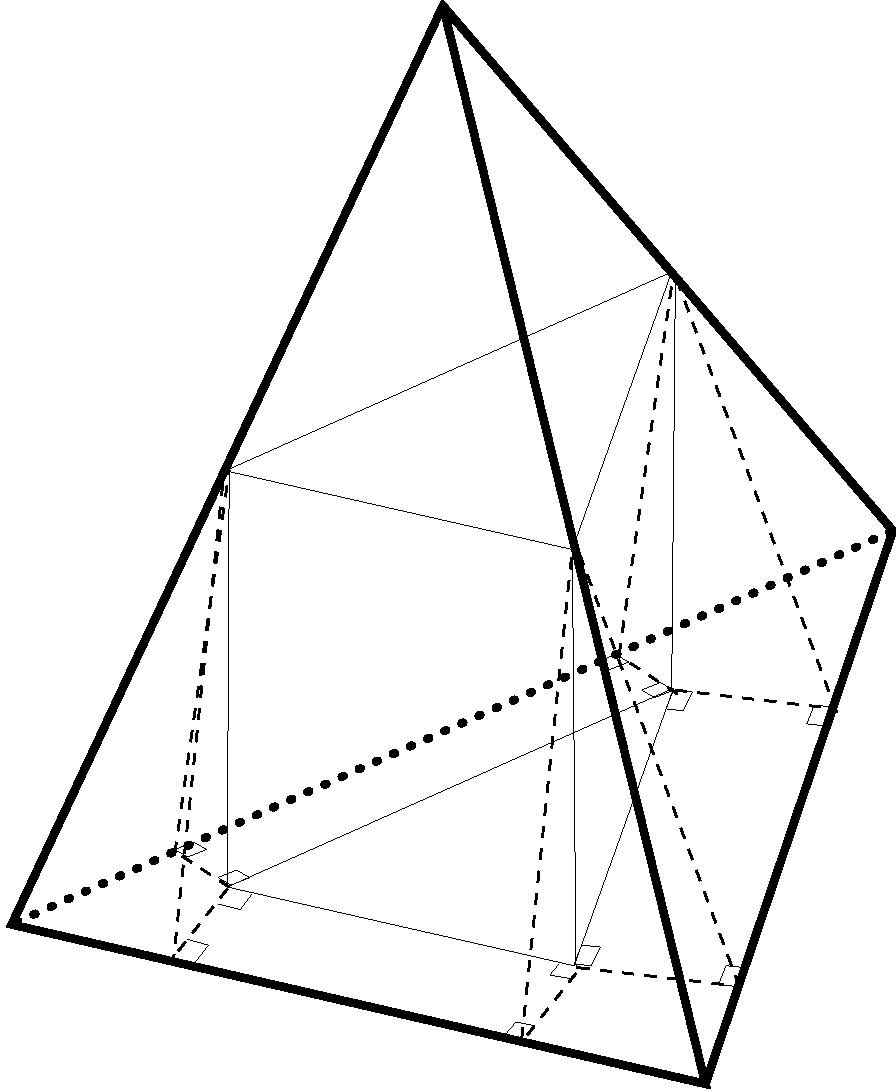
\includegraphics[width=90mm]{figs/pyr.pdf}
%     \end{center}
% \label{pyramid}
% \end{figure}


% Here is an example of using the macros
% \verb2\singlespacing2 and \verb2\doublespacing2:

% \singlespacing	% <------------------------------

% This paragraph was preceded by the
% command \verb2\singlespacing2.
% See the Specifications of the Grad School for instructions
% about when single spacing is appropriate in a thesis.

% \doublespacing	% <------------------------------

% And now, here is an example of using the macros
% \verb2\begin{singlespace}2 and \verb2\end{singlespace}2;
% another way to get single-spacing.

% \begin{singlespace}	% <-----------------------------
% Two cases are studied in the present work which differ only in the
% boundary conditions.  Each different boundary condition model a
% different source of instability.  The boundary of the first case
% consists of a steady, axisymmetric sidewall radial velocity boundary
% and a time-dependent, non-axisymmetric endwall axial velocity
% boundary.  The second case is studied with a fixed impermeable axial
% velocity along the endwall and a combination axisymmetric steady and
% non-axisymmetric unsteady radial velocity along the sidewall.
% \end{singlespace}	% <-----------------------------


% Usually you want to use a table produced by some other
% software, such as Excel, rather than try to do it using
% \LaTeX macros.  If the table is saved/printed to a PDF file,
% then it can be displayed using the
% $\backslash${\tt includegraphics} macro
% inside a {\tt table} environment:


% \begin{table}
%     \caption[Table from a PDF file]{
% 	This table wasn't constructed with \LaTeX{}
% 	commands, but resides in PDF file
% 	({\tt tableD.pdf})
% 	created by some other software.
% 	}
%     \begin{center}
% 	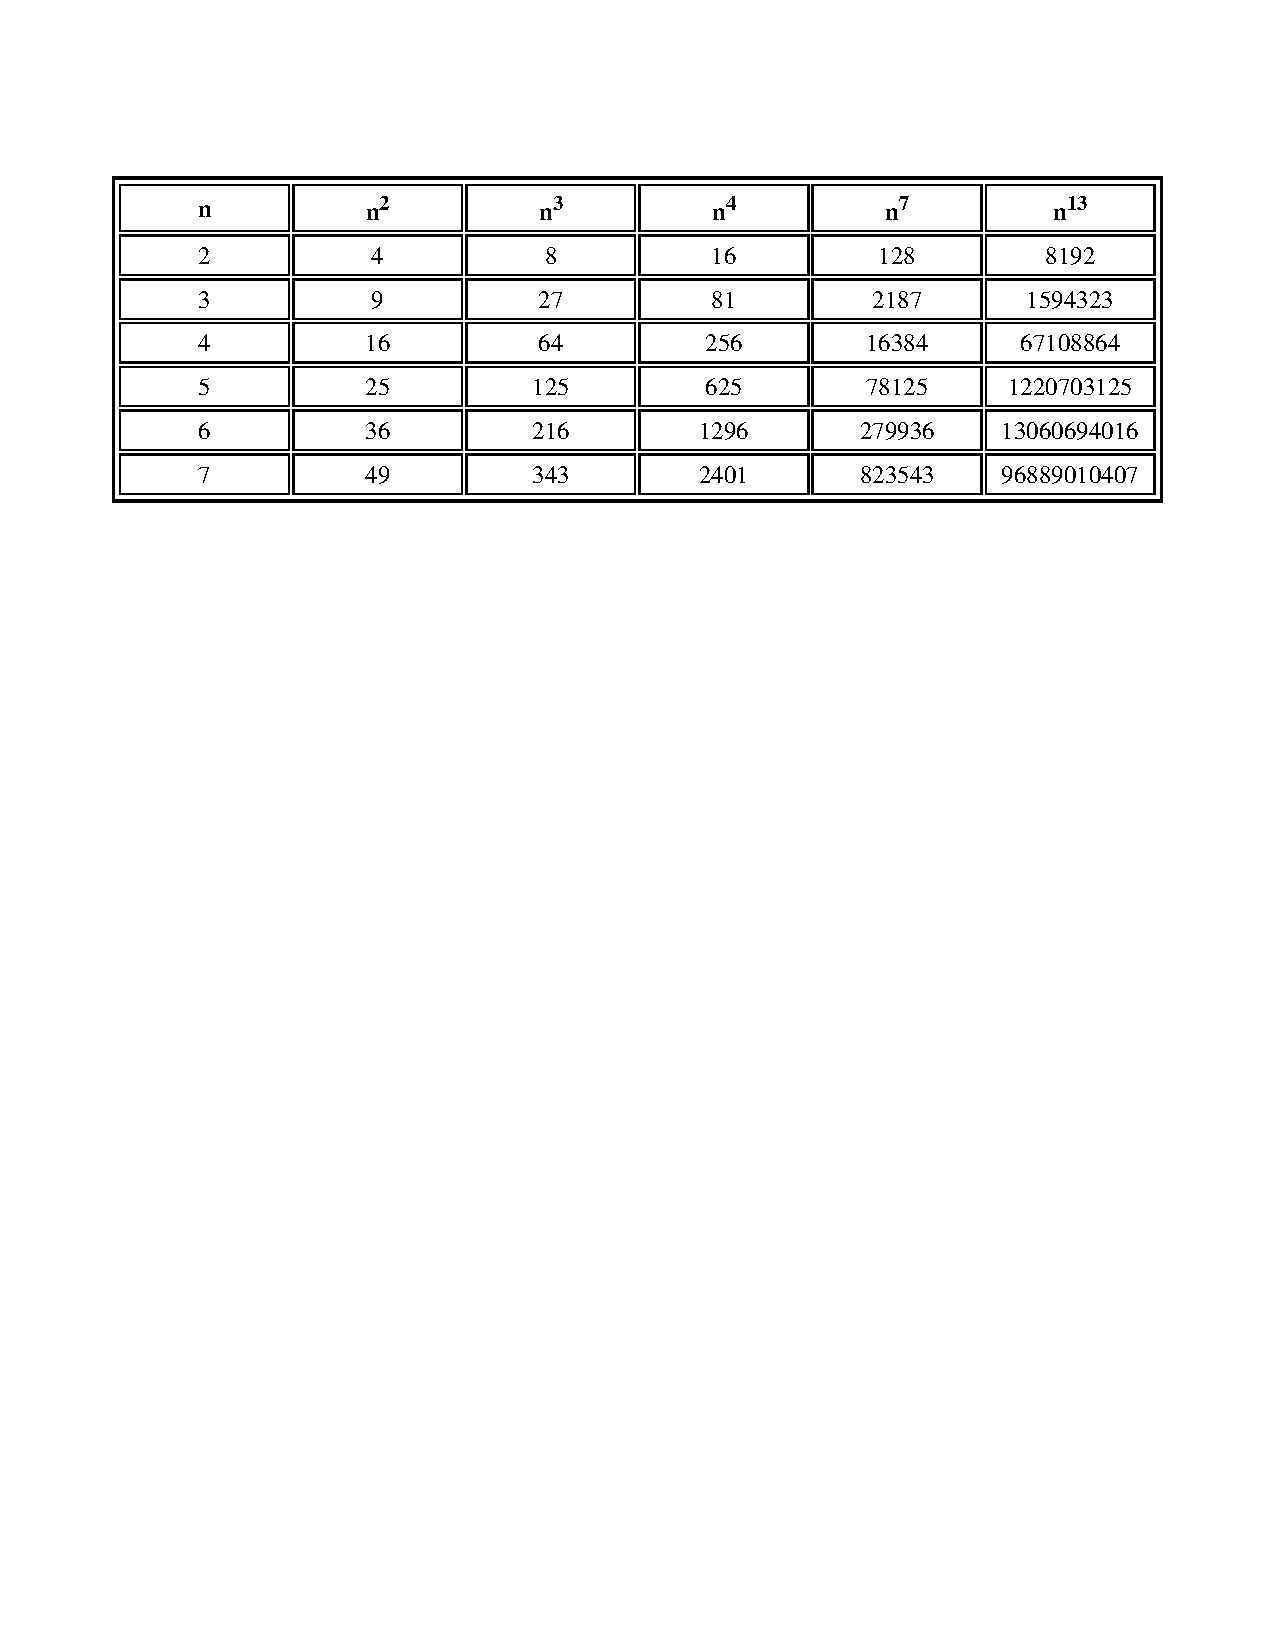
\includegraphics[width=5.45in]{figs/tableD.pdf}
%     \end{center}
% \label{pdftable}
% \end{table}


% Some of the boundary conditions are:

% \begin{eqnarray}
%   z=0; && V_z = \twochoices
% 	{0, && t\leq0}
% 	{\widetilde{F}_{zw}(r,\theta,t), && t>0}
% 						\label{eq:endwall} \\
%   z=0; && V_{\theta}=V_r=0			\label{eq:endnoslip} \\
%   r=0; && P,\rho,T,V_r,\vth,V_z~\mbox{finite},	\label{eq:centerline} \\
%   r=1; && V_r= F_{rws}(z),			\label{eq:injection} \\
%   r=1; && V_z=\vth =0,				\label{eq:sidenoslip}
% \end{eqnarray}
% and solutions must be periodic in $\theta$.

% If you don't believe this stuff, check out
% Mulick\cite{mulick} and Baylor\cite{baylor}.


% \section{Yet another section}

% \subsection{
% 	Just meaningless text to test lines per page
% 	\label{ss}}

% According to the Grad School specs.   there should be 24--27 lines
% of print per page of a thesis.  This should be true whether the font
% size is 10, 11, or 12.  Count them up; does this document conform?
% According to the Grad School specs.   there should be 24--27 lines
% of print per page of a thesis.  This should be true whether the font
% size is 10, 11, or 12.  Count them up; does this document conform?
% According to the Grad School specs.   there should be 24--27 lines
% of print per page of a thesis.  This should be true whether the font
% size is 10, 11, or 12.  Count them up; does this document conform?
% According to the Grad School specs.   there should be 24--27 lines
% of print per page of a thesis.  This should be true whether the font
% size is 10, 11, or 12.  Count them up; does this document conform?
% According to the Grad School specs.   there should be 24--27 lines
% of print per page of a thesis.  This should be true whether the font
% size is 10, 11, or 12.  Count them up; does this document conform?
% According to the Grad School specs.   there should be 24--27 lines
% of print per page of a thesis.  This should be true whether the font
% size is 10, 11, or 12.  Count them up; does this document conform?
% According to the Grad School specs.   there should be 24--27 lines
% of print per page of a thesis.  This should be true whether the font
% size is 10, 11, or 12.  Count them up; does this document conform?
% According to the Grad School specs.   there should be 24--27 lines
% of print per page of a thesis.  This should be true whether the font
% size is 10, 11, or 12.  Count them up; does this document conform?
% According to the Grad School specs.   there should be 24--27 lines
% of print per page of a thesis.  This should be true whether the font
% size is 10, 11, or 12.  Count them up; does this document conform?
% According to the Grad School specs.   there should be 24--27 lines
% of print per page of a thesis.  This should be true whether the font
% size is 10, 11, or 12.  Count them up; does this document conform?
% According to the Grad School specs.   there should be 24--27 lines
% of print per page of a thesis.  This should be true whether the font
% size is 10, 11, or 12.  Count them up; does this document conform?
% According to the Grad School specs.   there should be 24--27 lines
% of print per page of a thesis.  This should be true whether the font
% size is 10, 11, or 12.  Count them up; does this document conform?
% According to the Grad School specs.   there should be 24--27 lines
% of print per page of a thesis.  This should be true whether the font
% size is 10, 11, or 12.  Count them up; does this document conform?
% According to the Grad School specs.   there should be 24--27 lines
% of print per page of a thesis.  This should be true whether the font
% size is 10, 11, or 12.  Count them up; does this document conform?
% According to the Grad School specs.   there should be 24--27 lines
% of print per page of a thesis.  This should be true whether the font
% size is 10, 11, or 12.  Count them up; does this document conform?
% According to the Grad School specs.   there should be 24--27 lines
% of print per page of a thesis.  This should be true whether the font
% size is 10, 11, or 12.  Count them up; does this document conform?
% According to the Grad School specs.   there should be 24--27 lines
% of print per page of a thesis.  This should be true whether the font
% size is 10, 11, or 12.  Count them up; does this document conform?

% \paragraph{What is it?}
% This is a labelled paragraph.
% The heading of the paragraph is emphasized.
% This is a labelled paragraph.
% The heading of the paragraph is emphasized.

% \subsection{This is a subsection}

% This is a subsection.
% Filler filler filler filler filler filler filler filler.
% Filler filler filler filler filler filler filler filler.

% \subsection{This is another subsection}

% This is another subsection.
% Filler filler filler filler filler filler filler filler.
% Filler filler filler filler filler filler filler filler.

% \paragraph{This is paragraph number 2.}
% It used a \verb2\paragraph{}2 header, which
% are always inlined (with extra space)
% and  boldfaced.

% This is the third paragraph of the subsection.
% Filler filler filler filler filler filler filler filler.
% Filler filler filler filler filler filler filler filler.

% %%%%%%%%%%%%%%%%%%%%%%%%%%%%%%%%%%%%%%%%%%%%%%%%%%%%%%%%%%

% \subsubsection{This is a subsubsection (1)}
% This is the first paragraph of the subsubsection.
% Whether it is numbered or inlined depends on the
% option selected at the beginning of the
% thesis.

% By default, a \verb2\subsubsection2 heading is numbered
% and set off on a separate line, left-justified.

% \paragraph{However.}
% Using the \verb2inlineh42 option, subsubsection headers
% are inlined.
% And using the \verb2nonumh42 option suppresses
% numbering of the subsubsections.
% Together they make subsubsection headings
% just the same as paragraph headings.


% %%%%%%%%%%%%%%%%%%%%%%%%%%%%%%%%%%%%%%%%%%%%%%%%%%%%%%%%%%

% \subsubsection{
% 	This is another subsubsection (2)
% 	\label{sss}
% 	}

% Once again, whether its heading is numbered
% and/or inlined depends on the class options
% chosen at the start.

% There is no ``subsubsubsection'' entity,
% and ``subparagraph'' gets no special treatment
% in \emph{thesis} class.

% \section{The End}
% \label{sec:end}

% Finally, this is the end.  The bibliography starts on
% the next page.
% Note how the \verb2\hyperref2 package
% (mentioned in chapter \ref{introchap})
% also makes hyperlinks from references
% (e.g., Mulick\cite{mulick})
% to entries in the bibliography.

